\subsection{Interfaccia - Barre degli Strumenti}

\begin{frame}

  \frametitle{Interfaccia - Barra Inferiore}
  
  \begin{textblock*}{20cm}(0.2cm,1.75cm)
    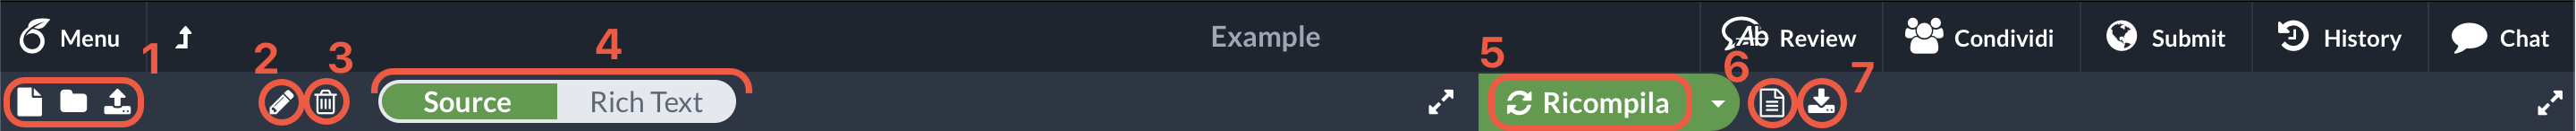
\includegraphics[scale=0.245]{over5_inf}
  \end{textblock*}

  \begin{textblock*}{20cm}(1cm,3.1cm)
    Come potete vedere ci sono due barre.\newline
    Quella Inferiore presenta appositi comandi per:\newline
    \begin{enumerate}
       \item Nuovo File / Nuova Cartella / Carica
       \item Rinomina File
       \item Elimina File
       \item Passaggio fra Source Text e Rich Text (con apposite funzionalità)
       \item Comando Compile e relative opzioni
       \item File di Log
       \item Scarica PDF
    \end{enumerate}
  \end{textblock*}
  

\end{frame}

\begin{frame}

  \frametitle{Interfaccia - Barra Superiore}
  
  \begin{textblock*}{20cm}(0.2cm,1.75cm)
    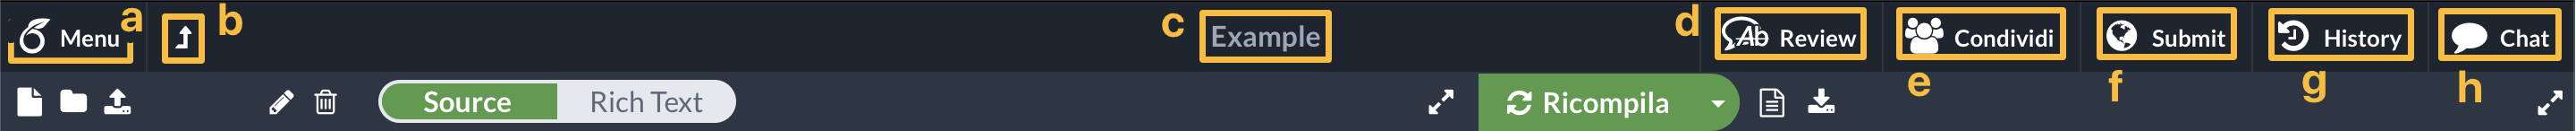
\includegraphics[scale=0.245]{over5_sup}
  \end{textblock*}

  \begin{textblock*}{20cm}(1cm,3.1cm)
    La barra Superiore permette di:\newline
    \begin{enumerate}[a)]
       \item Accedere alle funzionalità del Menù
       \item Tornare alla lista dei progetti
       \item Vedere il nome del file corrente
       \item Aprire la finestra di Revisione
       \item Condividere il progetto con un altro account Overleaf
       \item Effettuare il Submit ad alcuni gruppi Overleaf
       \item Vedere lo storico dei cambiamenti (utile per progetti condivisi)
       \item Aprire la Chat (utile per progetti condivisi)
    \end{enumerate}
    \end{textblock*}

\end{frame}

\begin{frame}

  \frametitle{Interfaccia - Consigli Utili}

    \begin{itemize}
       \item Dal Menù è possibile scaricare anche il codice sorgente, non solo il PDF
       \item È possibile anche sincronizzare il progetto con DropBox, Git e GitHub
       \item Spesso, se si importano progetti di grandi dimensioni, Overleaf non è in grado
       di riconoscere correttamente il documento principale (quello da cui far partire la compilazione).
       È necessario quindi controllare che questo sia specificato correttamente nella sezione \textbf{Documento
       Principale} del Menù
       \item Il tasto \textbf{Ricompila} presenta delle funzionalità utili. Quella più degna di nota è l'
       \textit{Auto compile}, la quale, se settata su \texttt{On} permette di visualizzare le modifiche al
       codice sorgente in real-time sul PDF generato
    \end{itemize}

\end{frame}





